
\chapter{介绍}

在早期的人工智能中,我们处理和解决对人类来说难处理,但对机器来说很简单的,可以用正式的数学规则描述的问题。
而人工智能真正的挑战是那些对人类来说很简单,但难以正式的描述出的问题,比如识别说出的话或者图片中的人脸。

解决办法就是让机器从数据中进行学习,并以结构化的概念来理解这个世界,每个概念通过与更简单的概念的关系来定义。
如果我们画一个图来描述这些概念是如果在其他概念上构成的,该图就会很深,有很多层。
因此,也叫做深度学习。

最早的人工智能解决方式为:硬编码知识(hard-code knowledge)。
这种方式有一个知识库和一个推理机,
推理机由一系列逻辑推理规则组成,(人为设定)
通过将推理机应用与知识库来对世界进行理解,
这种方式未取得很大的成成功。



hard-code knowledge面临的难题是,AI系统需要有能力来获取知识,通过从原始数据中提取模式(pattern)。
这种能力就是机器学习。
一个简单的机器学习的算法为逻辑回归。


这些简单的机器学习算法的效率很大程度上依赖于数据的表征(representation),
表征中的每一个信息都称为特征(feature),
比如 [身高,体重,年龄,血压,心率...],
表征的选择对机器学习的效率有巨大的影响。

然而对于许多任务来说,我们很难知道需要提取什么特征。
比如,我们想识别图片中的汽车,我们可以使用汽车有轮子这个特征,但我们很难用像素来描述轮子,一个轮子有几何形状,但照片中的轮子受到光照,阴影,挡板和前景的障碍物的遮挡等等的影响。


一个解决方法为,使用机器学习来同时学习表征到输出的映射和表征本身,这个方法叫做“表征学习”。
学习得到的表征常常比手动设计的表征的准确率要高。
表征学习的经典算法为自编码器(autoencoder),
自编码器由编码函数(将输入数据转化为不同的表征)和解码函数(将新的表征转化为原始数据格式)组成。


当我们设计特征或者算法来学习特征的时候,我们的目标通常是将变量的因素(factors of variation)进行分离,而这因素可以解释观察到的数据。
在此处,因素指单独的影响源,该因素不是混合的,
它们可以被想象为我们用来理解数据中的复杂变化性的一种概念或者抽象,
例如,当我们分析一段录音,因素包括说话这的年龄,性别,口音和说话的内容等,
当我们分析汽车的照片,因素有汽车的位置,颜色,角度和太阳的亮度等。

一个主要的问题为,许多变量的因素同时影响着我们观测到的数据中的所有单个部分。
比如,红色轿车图片中的色素在晚上的时候非常接近黑色,阳光对整张图有着影响。

当然,我们很难从数据提取出高层次的抽象特征,比如口音,这需要对数据有专业的,人类水平的理解。
当获取表征的难度和解决问题的难度相似的时候,表征学习似乎对我们是没有帮助的。


深度学习通过引入使用更简单的表征表示的表征来解决表征学习中的核心问题。
深度学习是机器可以从更简单的概念中构建出更复杂的概念。
经典的深度学习算法为,“前馈深度网络”(feedforward deep network)或者多层感知机(multilayer perception)。


从基于规则的系统 $\rightarrow$ 机器学习 $\rightarrow{}$ 表征学习 $\rightarrow{}$ 深度学习的进化如图\ref{fig:introduction-deep-learning}所示:
\begin{figure}[!ht]
  \centering
  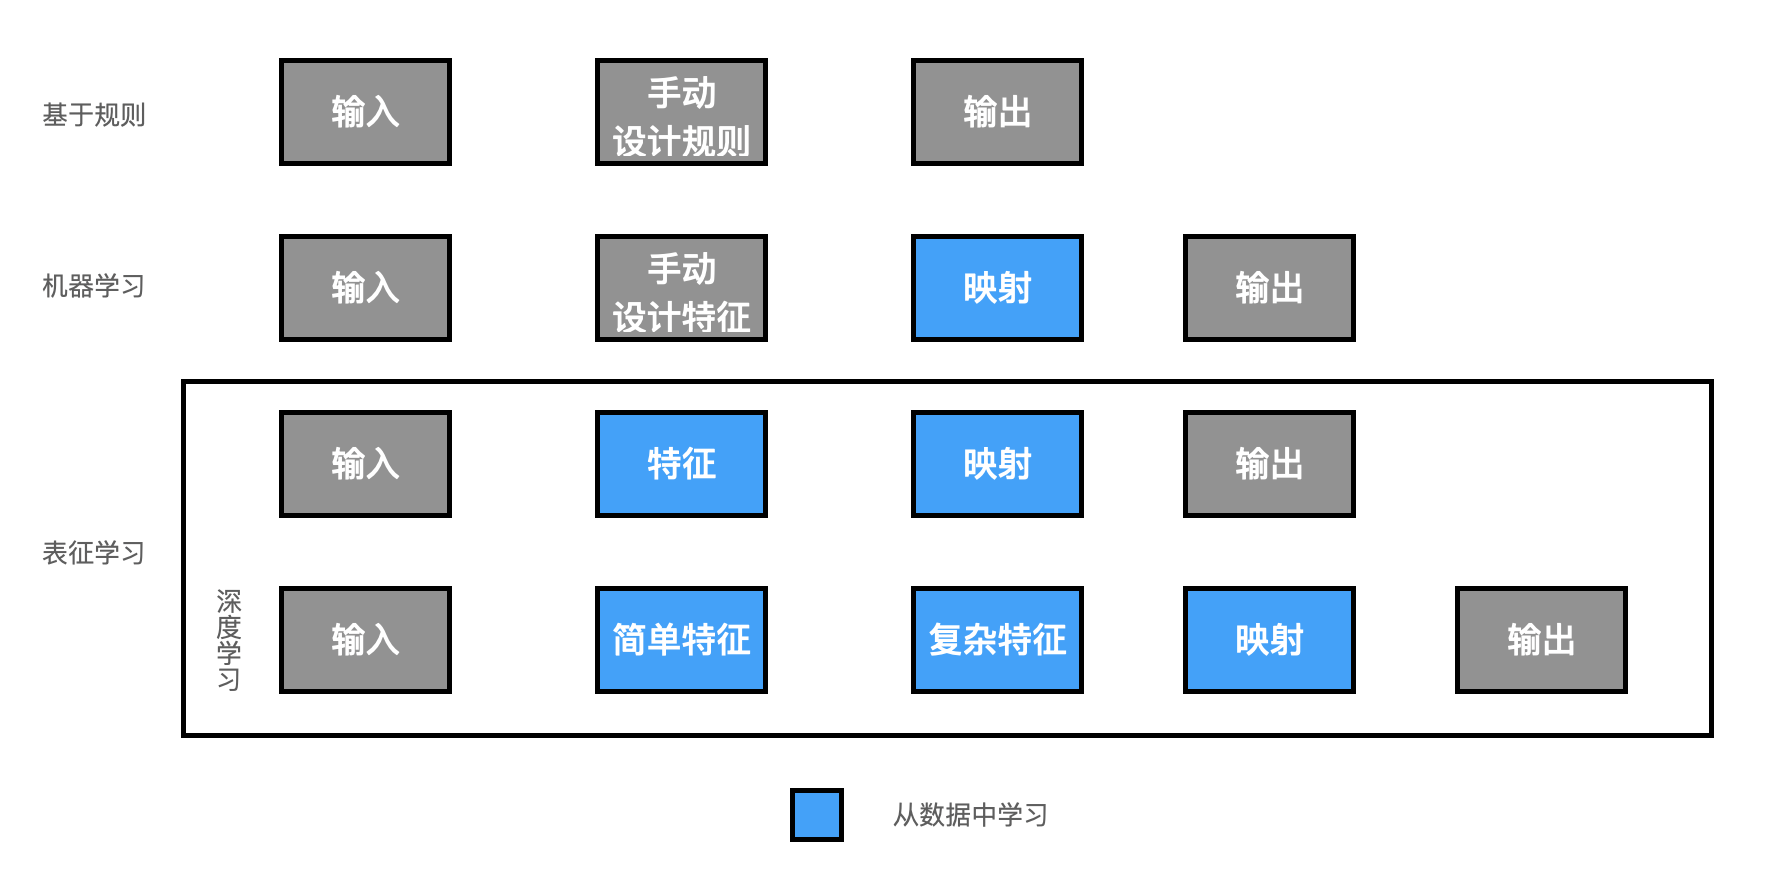
\includegraphics[width=\textwidth]{introduction-deep-learning.png}
  \caption{深度学习的进化}
  \label{fig:introduction-deep-learning}
\end{figure}






